% coding:utf-8

%FOSAET, a LaTeX-Code for a electrical summary of basic electronics
%Copyright (C) 2013, Daniel Winz, Ervin Mazlagic

%This program is free software; you can redistribute it and/or
%modify it under the terms of the GNU General Public License
%as published by the Free Software Foundation; either version 2
%of the License, or (at your option) any later version.

%This program is distributed in the hope that it will be useful,
%but WITHOUT ANY WARRANTY; without even the implied warranty of
%MERCHANTABILITY or FITNESS FOR A PARTICULAR PURPOSE.  See the
%GNU General Public License for more details.
%----------------------------------------

\newpage
\section{Quellenverschiebung}
Das Verschieben von Quellen kann notwendig sein, wenn zum Beispiel beim Knotenpotentialverfahren eine ideale Spannungsquelle nicht in eine Stromquelle umgewandelt werden kann. 

\subsection{Verschiebung von Spannungsquellen}
\begin{enumerate}
  \item Knoten bestimmen, über welchen die Spannungsquelle verschoben werden soll. 
  \item Spannungsquelle vervielfachen und über Knoten verschieben. \\
  Dabei muss die Spannungsquelle auf jede Leitung verschoben werden, welche zum Knoten führt. Somit werden die Maschengleichungen nicht verändert. 
\end{enumerate}
% Spannungsquellen können über einen Knoten hinweg geschoben werden. Bei der Verschiebung muss er vervielfacht werden und auf jede andere Leitung am Knoten eingefügt werden. 
\begin{figure}[h!]
	\centering
	\begin{subfigure}[b]{0.4\textwidth}
		\centering
		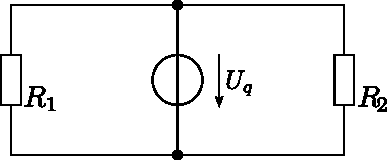
\includegraphics[scale=\schscalesmall]{qversch_uq1_sch.pdf}
% 		\caption{1}
		\label{sch:starqversch_uq1}
	\end{subfigure}
	\begin{subfigure}[b]{0.4\textwidth}
		\centering
		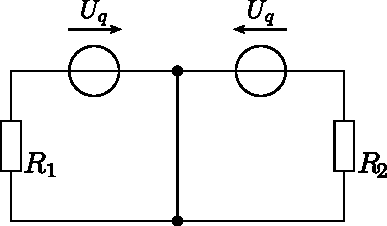
\includegraphics[scale=\schscalesmall]{qversch_uq2_sch.pdf}
% 		\caption{2}
		\label{sch:qversch_uq2}
	\end{subfigure}
	\caption{Verschiebung von Spannungsquellen}
	\label{sch:qversch_uq1}
\end{figure}

\newpage
\subsection{Verschiebung von Stromquellen}
\begin{enumerate}
  \item Masche bestimmen, innerhalb welcher die Stromquelle verschoben werden soll. 
  \item Stromquelle vervielfachen. 
  \item Stromquellen verschieben, dass zwischen jedem Knoten ausser an der Stelle der vorherigen Stromquelle eine Stromquelle zu liegen kommt. 
\end{enumerate}
% Stromquellen werden zunächst vervielfacht und anschliessend innerhalb der Masche an jeden Knoten "umgehängt". 
\begin{figure}[h!]
	\centering
	\begin{subfigure}[b]{0.3\textwidth}
		\centering
		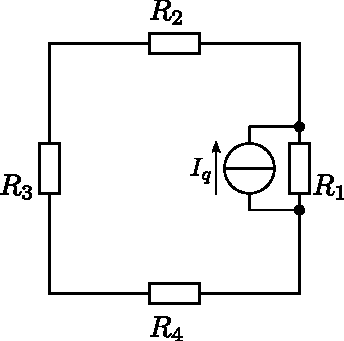
\includegraphics[scale=\schscalesmall]{qversch_iq1_sch.pdf}
% 		\caption{1}
		\label{sch:qversch_iq1}
	\end{subfigure}
	\begin{subfigure}[b]{0.3\textwidth}
		\centering
		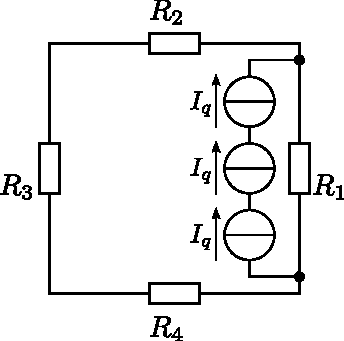
\includegraphics[scale=\schscalesmall]{qversch_iq2_sch.pdf}
% 		\caption{2}
		\label{sch:qversch_iq2}
	\end{subfigure}
	\begin{subfigure}[b]{0.3\textwidth}
		\centering
		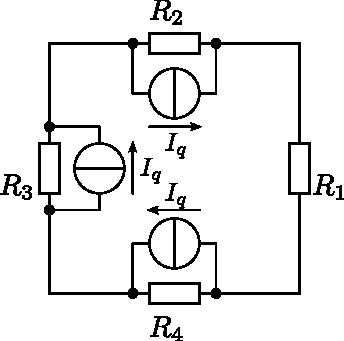
\includegraphics[scale=\schscalesmall]{qversch_iq3_sch.pdf}
% 		\caption{3}
		\label{sch:qversch_iq3}
	\end{subfigure}
	\caption{Verschiebung von Stromquellen}
	\label{sch:qversch_iq}
\end{figure}
